\documentclass{article}
\usepackage{tikz}
\usetikzlibrary{arrows.meta,positioning,calc,shapes.geometric}
\pagestyle{empty}
\begin{document}
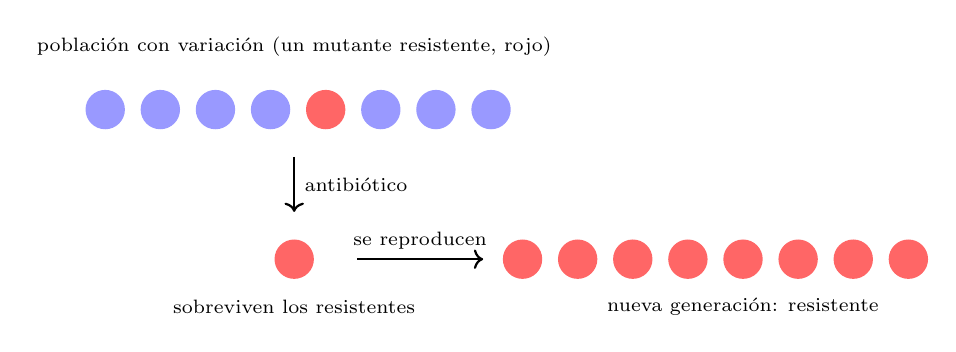
\begin{tikzpicture}

\foreach \i/\c in {0/blue!40,1/blue!40,2/blue!40,3/blue!40,4/red!60,5/blue!40,6/blue!40,7/blue!40} {\fill[\c] (0.6+\i*0.7,2.6) circle (0.25);}
\node[font=\scriptsize] at (3.0,3.4) {población con variación (un mutante resistente, rojo)};
\draw[->, thick] (3.0,2.0) -- (3.0,1.3) node[midway, right, font=\scriptsize] {antibiótico};
\fill[red!60] (3.0,0.7) circle (0.25); \node[font=\scriptsize] at (3.0,0.1) {sobreviven los resistentes};
\draw[->, thick] (3.8,0.7) -- (5.4,0.7) node[midway, above, font=\scriptsize] {se reproducen};
\foreach \i in {0,1,2,3,4,5,6,7} {\fill[red!60] (5.9+\i*0.7,0.7) circle (0.25);}
\node[font=\scriptsize] at (8.7,0.1) {nueva generación: resistente};

\end{tikzpicture}
\end{document}
